\subsection{The Search and the Execution loop}%
\label{subsec:two_loops}
Now that \ac{hgraph} is defined let's find out how it reacts to various behaviour. The reaction of the \ac{hgraph} can be visualized in a flowchart of the \ac{hgraph} provided in \cref{tikz:flowchart_hgraph}. In \cref{tikz:flowchart_hgraph} two loops can be identified, clarified in \Cref{fig:two_loops_identified}. In the search, loop hypotheses are formed and the execution loop tests the hypothesis.\bs

\begin{figure}[H]
    \centering
    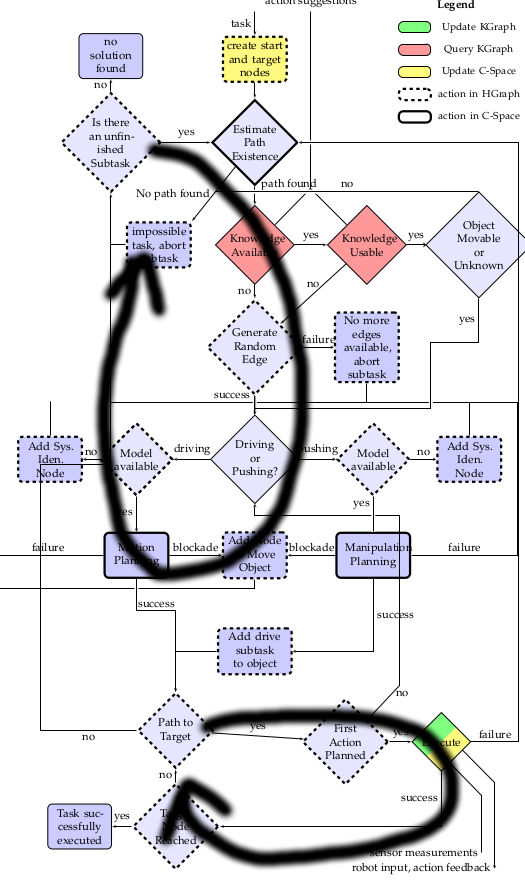
\includegraphics[width=5cm]{figures/two_loops_identified}
    \caption{The search and execution loop.}%
    \label{fig:two_loops_identified}
\end{figure}
\todo[inline]{Update figure above, professionalise arrows}

While the \ac{hgraph} resides in the search loop, hypotheses are formed. Forming a hypothesis, generating edges, nodes and progressing their status as described in \cref{tikz:status_identification_edge,tikz:status_action_edge} respectively. The \ac{hgraph} operates synchronously, thus at any point in time, the \ac{hgraph} resides in a single block within \cref{tikz:flowchart_hgraph}. The result is that the robots cannot operate whilst the \ac{hgraph} resides in the search loop, and during execution, no hypothesis can be formed or updated. Assumption~\ref{assumption:closed_world} guarantees that the robot environment does not change causing existing hypotheses to be outdated.\bs

While the \ac{hgraph} resides in the execution loop, \textit{an edge is being executed}. The phrase \quotes{an edge is being executed} seems odd at first because every aspect of closed-loop control resides in an edge, edges can be executed. Recall that nodes in the \ac{hgraph} represent objects in a state, and edges represent actions. Now a flowchart of the behaviour of the \ac{hgraph} is presented.\bs

% \newgeometry{left=1.1cm,bottom=0.1cm,top=1.9cm,headsep=0.1in,heightrounded}

\newpage
\vspace*{-1.2cm}
\hspace{-1.2cm}
\begin{minipage}{10cm}
\begin{figure}[H] 
\centering
\begin{tikzpicture}]
  [node distance = 3cm] 

    % Nodes
    \node [block, fill=yellow!50, line width=2pt, dashed] (first) {Create Start and Target Nodes};
    
    % legend
    \node[text width=2.8cm, yshift=0.6cm, right of=first, node distance=7cm, text centered, rounded corners, minimum height=1em, label={[name=lab, yshift=0.4cm, left]\textbf{Legend}}] (legend1) {\small Update KGraph};
    \node[rectangle, draw, left of=legend1, fill=green!50, rounded corners, minimum height=1em, minimum width=1cm, node distance=2cm] (legend1color) {};
    
    \node[text width=2.8cm, below of=legend1, text centered, minimum height=1em, node distance=0.7cm] (legend2) {\small Query KGraph};
    \node[rectangle, draw, left of=legend2, fill=red!40, rounded corners, minimum height=1em, minimum width=1cm, node distance=2cm] (legend2color) {};
   
    \node[text width=2.8cm, below of=legend2, text centered, minimum height=1em, node distance=0.7cm] (legend3) {\small Update C-Space};
\node[rectangle, draw, left of=legend3, fill=yellow!50, rounded corners, minimum height=1em, minimum width=1cm, node distance=2cm] (legend3color) {};
    
    \node[text width=2.8cm, below of=legend3, text centered, minimum height=1em, node distance=0.7cm] (legend4) {\small action in HGraph};
    \node[rectangle, draw, left of=legend4, rounded corners, minimum height=1em, minimum width=1cm, node distance=2cm, line width=2pt, dashed] (legend4color) {};
 
    \node[text width=2.8cm, below of=legend4, text centered, minimum height=1em, node distance=0.7cm] (legend5) {\small action in C-Space};
\node[rectangle, draw, left of=legend5, rounded corners, minimum height=1em, minimum width=1cm, node distance=2cm, line width=2pt] (legend5color) {};

    % nodes, Path exists 
    \node [decision, below of=first, node distance=2.6cm, line width=2pt] (path_existence) {Estimate Path Existence};
    \node [decision, left of=path_existence, node distance=4.5cm, line width=2pt, dashed] (subtasks) {Is There an Unfinished Subtask};

    \node [block, above of=subtasks, node distance=2.8cm] (no_solution_found) {Task Finished};
    
    % nodes, Knowledge available
    \node [decision, fill=red!40, below of=path_existence, node distance=3.2cm, inner sep=0.5mm] (know_avail) { Knowledge Available };
    \node [decision, fill=red!40, right of=know_avail, node distance=3.5cm, inner sep=0.5mm] (know_good) {Knowledge Usable};
    \node [decision, right of=know_good, node distance=3.5cm, text width=1.7cm] (movable) {\vspace{0.1cm}\shortstack[]{Object\\Movable or\\Unknown}};
    \node [block, left of=know_avail, node distance=3cm, line width=2pt, dashed] (impossible) {Impossible Node};
    
    % nodes, Generate new edge
    \node [decision, below of=know_avail, node distance=3.2cm, line width=2pt, inner sep=0.5mm, dashed] (goto_sys_iden) {Generate Random Action};

    \node[block, right of=goto_sys_iden, node distance=3.5cm, line width=2pt, dashed] (no_trans_found) {All Possible Actions Failed};
    
    
    % Motion/Manipulation planning 
    \node [decision, below of=goto_sys_iden, node distance=3.5cm] (single_multi) {Action Type};

    \node [decision, line width=2pt, dashed, left of=single_multi, node distance=3.7cm] (model_avail_single) {Model Available};
    \node [decision, line width=2pt, dashed, right of=single_multi, node distance=3.7cm] (model_avail_multi) {Model Available};
    \node [block, line width=2pt, dashed, left of=model_avail_single, node distance=2.8cm] (sys_iden_single) {Add Drive Sys. Iden. Node};
    \node [block, line width=2pt, dashed, right of=model_avail_multi, node distance=2.8cm] (sys_iden_multi) {Add Push Sys. Iden. Node};
    \node [block, line width=2pt, dashed, below of=single_multi, node distance=2.7cm] (move_object) {Add Node to Move Object};
    \node [block, line width=2pt, left of=move_object, node distance=3.7cm] (motion_planning) {Motion Planning};
    \node [block, line width=2pt, right of=move_object, node distance=3.7cm, text width=2.1cm] (manipulation_planning) {Manipulation Planning};

    \node [decision, line width=2pt, dashed, minimum width=2.3cm, below of=move_object, node distance=2.3cm, xshift=1.75cm] (drive_to_push_position) {Robot Close to Push Pose};
    \node [block, line width=2pt, dashed, minimum width=2.3cm, below of=move_object, node distance=2.3cm, xshift=-1.75cm] (goto_push_position) {Add Node to Drive to Push Pose};
  
    \node [decision, line width=2pt, above of=sys_iden_single, node distance=3.5cm] (add_drive_node) {Robot Close to Object};

    \node [block, dashed, line width=2pt, above of=add_drive_node, node distance=3.2cm] (do_add_drive_node) {Add Node to Drive to Object};

    % nodes, Path to target
    \node [decision, below of=motion_planning, node distance=4.0cm, line width=2pt, dashed] (global_path) {Path to Target}; 
1   \node [decision, right of=global_path, node distance=7.4cm, line width=2pt, dashed] (first_action) {First Action Planned};

    \node [decision, right of=first_action, diagonal fill={yellow!50}{green!50}, node distance=3cm] (execute) {Execute};
     
    % nodes, Target node reached 
    \node [decision, below of=global_path, node distance=3cm, line width=2pt, dashed] (target_node_reached) {Target Node Reached};
    \node [block, left of=target_node_reached, node distance=3cm] (end) {Subtask Successfully Completed};
    
    % Edges
    \path[line] ++(0,1.2) -- node[yshift=0.2cm, above]{task} (first);
    \path[line] (first) -- node[midway](to_path_exists){}(path_existence); 
    
    % edges, Path exists 
    \path[line] ([xshift=0.2cm, yshift=-0.2cm] path_existence.south west) -| node[near start, xshift=-0.4cm, above] {no path found} (impossible.north);
    \path[line] (subtasks.north) --  node[left] {no} (no_solution_found);
    \path[line] (path_existence) -- node[xshift=0cm, yshift=0.15cm, left] {path found} (know_avail); 
    \path[line] (subtasks.east) -- node[above] {yes} (path_existence.west);
    
    % edges, Knowledge available
    \path[line] (know_avail) -- node[above] {yes} (know_good); 
    \path[line] (know_good) -- node[yshift=0.1cm, above] {no} (goto_sys_iden); 
    \path[line] (know_avail) -- node[left](toward_new_trans) {no} (goto_sys_iden); 
    \draw[-stealth] (know_good.east) -- node[above] {yes} (movable.west);
    
    % \draw[-]  ([xshift=3.2mm]toward_new_trans.center) -| node[near start, above] {no} (know_good.south);
    \draw[-](impossible.west) -- +(-0.47,0); 
     
    \draw[-]  ([xshift=2.75cm, yshift=6.6cm]know_avail.center) --  node[at start, above] {\shortstack[]{action\\suggestions}} ([xshift=1.75cm, yshift=3.75cm]know_avail.center) -- ([xshift=1.75cm, yshift=3.75cm]know_avail.center);

    \draw[-stealth]  ([xshift=1.75cm, yshift=3.75cm]know_avail.center) --  ([xshift=1.75cm, yshift=1.75cm]know_avail.center) -- (know_avail.north east);
    \draw[-stealth]  ([xshift=1.75cm, yshift=1.75cm]know_avail.center) -- (know_good.north west);
    \draw [draw=white,double distance=\pgflinewidth,ultra thick] (path_existence.east) -- +(2cm,0);
    
    % edges, Generate new edge
    \draw[-] (move_object.south) |- +(-7.70,-0.3);
    \draw [draw=white,double=black,double distance=\pgflinewidth,ultra thick] (motion_planning.south) -- +(0,-1cm);
    \draw[-stealth] (motion_planning.south)  -- ([yshift=-1cm]motion_planning.south) -| node[near start, left] {success} (global_path.north);
    \draw[-stealth] (manipulation_planning.south) |- node[near start, right] {success} (drive_to_push_position.east);
    \draw[-] ([xshift=0.1cm,yshift=0.1cm] drive_to_push_position.north west) -- node[at start, xshift=-0.5cm, above] {yes} ++(-4.75cm,0);
    \draw[-stealth] (drive_to_push_position.west) |- node[xshift=-0.3cm, above] {no} (goto_push_position.east);
    \draw[-] (goto_push_position.west) -- ++(-0.77cm, 0); 

    \draw[-] (motion_planning.west) -- node[above] {failure} +(-2.98,0);
    \draw[-] (manipulation_planning.east) -| node[near start, above] {failure} ([xshift=4.7cm,yshift=-0.6cm]no_trans_found.south) -- ([yshift=-0.6cm]no_trans_found.south);
    
    % edges, Single/Multi body
    \draw[-stealth] (single_multi.west) -- node[above] {driving} (model_avail_single);
    \draw[-stealth] (single_multi.east) -- node[above] {pushing} (model_avail_multi);
    \draw[-stealth] (model_avail_single.south) -- node[left] {yes} (motion_planning.north);
    \draw[-stealth] (model_avail_single.west) -- node[above] {no} (sys_iden_single);

    \draw[-stealth] (model_avail_multi.east) -- node[above] {no} (sys_iden_multi);
    \draw[-stealth] (motion_planning.east) -- node[above] {blockade} (move_object);
    \draw[-stealth] (manipulation_planning.west) -- node[above] {blockade} (move_object);
    \draw[-stealth] (goto_sys_iden) -- node[above] {fail} (no_trans_found);
    \draw[-] (sys_iden_single.north) --  ([yshift=0.56cm]sys_iden_single.north);
    \draw[-] (sys_iden_multi.north) |-  ([yshift=-0.6cm]no_trans_found.south);
    \draw[-] (no_trans_found.south) -- ++(0,-0.6cm) --([xshift=-8cm, yshift=-0.6cm]no_trans_found.south);
    \draw [draw=white,double=black,double distance=\pgflinewidth,ultra thick] (goto_sys_iden.south) -- node[yshift=0.1cm, right] {success}(single_multi.north);
    \draw[-stealth] ([yshift=0.05cm] goto_sys_iden.south) -- (single_multi.north);
    
    \draw[-] (movable.south) |- node[near start, left] {\shortstack[r]{yes, generate\\suggested\\edge}} ([xshift=-1.5cm, yshift=-1.4cm]movable.south) |- ([yshift=0.3cm]single_multi.north);
    \draw [draw=white,double distance=\pgflinewidth,ultra thick]  ([xshift=-1cm]movable.north) -- ([xshift=-7.2cm]movable.north);

    \draw[-] (movable.north) -- node[xshift=3cm, above]{no, object is obstacle}([xshift=-10cm]movable.north);
    % HERE
    \draw [draw=white,double=black,double distance=\pgflinewidth,ultra thick] ([xshift=5.5cm,yshift=0.3cm]single_multi.north) -- ([xshift=5.5cm, yshift=2cm]single_multi.north);
    % \draw[-] (know_good.east) -| node[above]{yes} ([xshift=5.5cm, yshift=0.2cm]single_multi.north) -- ([yshift=0.2cm]single_multi.north);

    
    \draw[-stealth] (add_drive_node.north) -- node[left] {no} (do_add_drive_node.south);
    \draw[-] (add_drive_node.north east) -- node[left] {yes} ++(1.3cm,1.3cm);
    \draw[-] (do_add_drive_node.east) --  ++(1.10cm,0);
    % edges, Path to target
    \path[line] (global_path) -- node[above] {yes} (first_action);
    \path[line] (first_action.east) -- node[above] {yes} (execute);
    \path[line] (global_path.west) -| node[xshift=1cm, left, above, near start] {no}  ([xshift=-2.8cm, yshift=8cm]global_path.west) -|  (subtasks.south); 
   
    \draw[-stealth] (first_action.north east) -- node[near end, left] {no} ([xshift=1.7cm, yshift=0.39cm]first_action.north) |- ([yshift=-0.35cm]single_multi.south) -- (single_multi.south);
    \draw [draw=white,double=black,double distance=\pgflinewidth,ultra thick] (manipulation_planning.east) -- +(1cm,0);
    \draw [draw=white,double=black,double distance=\pgflinewidth,ultra thick] (manipulation_planning.north) -- +(0,0.6cm);
    \draw [draw=white,double=black,double distance=\pgflinewidth,ultra thick] (single_multi.north west) -- ([xshift=1cm,yshift=-0.425cm] add_drive_node.south east);
    \draw[-stealth] (single_multi.north west) -- node[xshift=-0.7cm, yshift=0.4cm, near start, above, right] {identification} (add_drive_node.south east);

    \draw[-stealth] (model_avail_multi.south) -- node[near start, left] {yes} (manipulation_planning.north);
    
    \draw[-stealth] ([yshift=0.2cm, xshift=0.2cm]execute.south east) --  ([yshift=-0.8cm, xshift=1.2cm]execute.south east) -- node[at end, left] {robot input, action feedback} +(0,-2.7cm);
    
    \draw[stealth-] ([yshift=-0.2cm, xshift=-0.2cm]execute.south east) --  ([yshift=-1.2cm, xshift=0.8cm]execute.south east) -- node[left, at end] {sensor measurements} +(0, -1.8cm);
    
    \path[line] (execute.south) |- node[near start, left] {success} (target_node_reached.east);
    \draw[-stealth] (execute.east) -- node[above] {failure} ([xshift=1.5cm]execute.east) |- (path_existence.east);
    \draw[-] (end.north) -- ++(0,2.07cm);
    
    
    % edges, Target node reached 
    \path[line] (target_node_reached.north) -- node[left] {no} (global_path.south);
    \path[line] (target_node_reached.west) -- node[above] {yes} (end.east);

\end{tikzpicture}
% \vspace{-5cm}
\caption{Flowchart displaying the hypothesis graph's workflow.}%
\label{tikz:flowchart_hgraph}% 
\end{figure}

\end{minipage}
\newpage


\Cref{table:explainer_hgraph_figures_nodes} provides important information that does not fit on the flowchart above.


\begin{table}[H]
\centering
\rowcolors{2}{white}{my_light_blue}
\begin{tabular}[t]{>{\raggedright}p{3.5cm}>{\raggedright\arraybackslash}p{10.5cm}}
  \textbf{Node name} & \textbf{Description of actions taken}\\\toprule
  Task Finished & log all metrics for the \ac{hgraph}, then deconstruct \ac{hgraph}.\\
  Create Start and\newline Target Nodes & Generate a robot node and the start and target nodes for every subtask in the task.\\
Update Current Subtask & Select an unfinished subtask or update current subtask. Use a backward search, eleborated in \cref{subsec:connecting_nodes} so select and update the \textit{current\_start\_node} and \textit{current\_target\_node}. When all subtask have been addressed, conclude task is finished. \\
Estimate Path\newline Existence & Check if a path exists between \textit{current\_start\_node} and \textit{current\_target\_node} whilst assuming that the object is holonomic.\\
Add Node to\newline Drive to Object & Add a node before the \textit{current\_target\_node}.\\
Unfeasible Node & Update node's status to unfeasible because is can not be completed, log failed Edge.\\
Knowledge Available& Query the \ac{kgraph} for action suggestion to connect \textit{current\_target\_node} to \textit{current\_target\_node}\\
Knowledge Usable& Check if a suggested action is not on the blacklist.\\
Object Movable & Check if object is classified as movable\\
Robot Close to Object& Check if the object is inside directly reachable free space of the robot \\
Generate Random\newline Action& Randomly sample a controller with a compatible system identification method that is not on the blacklist. \\
All Possible Actions Failed & Every possible action is on the blacklist for the \textit{current\_target\_node}, update \textit{current\_target\_node} status to failed.\\
Add Drive System Identification Edge & Adds identification edge between a newly generated node and the drive action edge source node. \\
Model Available& Checks if the drive action edge contains a system model. \\
Action Type& Checks the action type. \\
Model Available& Checkif the push action edge containts a system model. \\
Add Push System\newline Identification Edge& Adds identification edge compatible with push action edge. \\
Motion Planning& Search a path for the \textit{current\_edge}, detect blocking objects. \\
Add Node to Free Path & Search closeby pose for object to free path. Create node to push object toward that pose. \\
Manipulation Planning & Search a path for the \textit{current\_edge}, detect blocking objects.\\
Add Node to Drive\newline to Push Pose& Create node to drive toward push pose, add before action edge. \\
Robot Close to\newline Push Pose & Check if the robot is overlapping with the best push position. \\
Path to Target& Is there a path from robot to target node in the \ac{hgraph}, then set first edge to \textit{current\_edge} otherwise update subtask.\\
First Action Planned&  Check if motion/manipulation planning was performed. \\
Execute& Execute the \textit{current\_edge}, update \ac{hgraph} after completion, log failed hypothesis if a fault is detected. \\
Subtask Succesfully\newline Completed& Log hypothesis metrics. \\
Target Node Reached& Check if the target node is reached.\\
\end{tabular}
\caption{Eleborated description of blocks in the \cref{pseudocode:proposed_rrt_star}, ordered in this table with respect the top to bottom, left to right it \cref{pseudocode:proposed_rrt_star}.}%
\label{table:explainer_hgraph_figures_nodes}
\end{table}

After initialising the \ac{hgraph} with a task, there is only a single access point toward the \ac{hgraph}. A function \textit{respond(observation)} that returns control input toward the robot. As argument function \textit{respond(observation)} takes an observation of the environment, such an observation contains measurements of every object's latest measured state. Recall that the perfect-sensor assumption, assumption~\ref{assumption:perfect_object_sensor} provides access to the exact states of every object.\bs
\todo[inline]{it is not clear to the reader that the text above only focusses on a single subtask AKA no global optimum for the task is sought}

\todo[inline]{Visualise this in hgraph: adding an edge for a drive action including sys iden. use "backward search"}
 A hypothesis is formed when the robot node is connected through a set of successive edges to the subtasks target node.
\todo[inline]{visualise this in hgraph: Executing a drive action}
\todo[inline]{Visualise this: adding an edge for a push action including sys iden.}
\todo[inline]{visualise this in hgraph: Executing a push action}
\todo[inline]{emphasise recursiveness of the hgraph, thus want to move box A, but B is in the way, move box B first, but box C is in the way, move box C first becomes: move(C) -> move(B) -> move(A)}

\todo[inline]{introduce the blacklist: a set of edges that cannot be added to a node because they failed in the past. The blacklist prevents regenerating edges which already failed in the past}

\todo[inline]{section about fault/monitoring metrics, that can halt and fail an executing edge}

What by now hopefully became clear to the reader is that the \ac{hgraph} autonomously searches for hypotheses to solve the task, one subtask at a time. The \ac{hgraph} switches between the search and execution loop. Switching from the search loop toward the execution loop when a hypothesis is found, and switching back when a hypothesis is completed or an action failed to complete.\bs

The limited number of possible edges (every combination of a system identification method with a compatible control method) guarantees that the robot tries to connect 2 nodes, but concludes that it cannot reach a node if all possible edges have failed. Eventually running out of nodes to connect and conclude that a subtask cannot be completed.\bs

In the next section, the edges that are executed will be reviewed and stored in a knowledge base. The knowledge base will suggest edges when faced with similar nodes to connect.
